%TEX-template borrowed from https://github.com/idlouhy/wonsole/blob/master/report/src/report.tex

\documentclass[12pt,a4paper,oneside]{report}

\usepackage[section] {placeins}

\usepackage[english]{babel}
\usepackage[utf8]{inputenc}
\usepackage[T1]{fontenc}
\usepackage{float}

\selectlanguage{english}

\usepackage[usenames,dvipsnames,svgnames,table]{xcolor}

\usepackage{graphicx}
\usepackage{tabu}
\usepackage{booktabs}
\usepackage{wrapfig}
\usepackage{pbox}
\usepackage{pgfplots}
\usepackage{pgfplotstable}
\usepackage{longtable}
\usepackage{pdfpages}

\usepackage{nameref}
\usepackage{fullpage}
\usepackage{verbatim}
\usepackage{url}
\usepackage{minitoc}
\usepackage{cite}
\usepackage{caption}
\usepackage{float}
\usepackage{color}
\usepackage{pgfgantt}
\usepackage{listings}
%\usepackage{xcolor}

\usepgfplotslibrary{dateplot}

\usepackage{tikz}
\usetikzlibrary{backgrounds}
\makeatletter

\usepackage{pdflscape}

\tikzset{%
  fancy quotes/.style={
    text width=\fq@width pt,
    align=justify,
    inner sep=2.5em,
    anchor=north west,
    minimum width=\textwidth,
  },
  fancy quotes width/.initial={.8\textwidth},
  fancy quotes marks/.style={
    scale=8,
    text=white,
    inner sep=0pt,
  },
  fancy quotes opening/.style={
    fancy quotes marks,
  },
  fancy quotes closing/.style={
    fancy quotes marks,
  },
  fancy quotes background/.style={
    show background rectangle,
    inner frame xsep=0pt,
    background rectangle/.style={
      fill=gray!25,
      rounded corners,
    },
  }
}

\newenvironment{fancyquotes}[1][]{%
\noindent
\tikzpicture[fancy quotes background]
\node[fancy quotes opening,anchor=north west] (fq@ul) at (0,0) {``};
\tikz@scan@one@point\pgfutil@firstofone(fq@ul.east)
\pgfmathsetmacro{\fq@width}{\textwidth - 2*\pgf@x}
\node[fancy quotes,#1] (fq@txt) at (fq@ul.north west) \bgroup}
{\egroup;
\node[overlay,fancy quotes closing,anchor=east] at (fq@txt.south east) {''};
\endtikzpicture}

\makeatother

\setlength{\parindent}{0.0in}
\setlength{\parskip}{1.5ex}

\setlength{\fboxsep}{0pt}
\setlength{\fboxrule}{1pt}

\fontfamily{ptm}\selectfont

\usepackage{hyperref}
\hypersetup{
    bookmarks=true,
    unicode=true,
    pdftoolbar=true,
    pdfmenubar=true,
    pdffitwindow=false,
    pdfstartview={FitH},
    pdftitle={Research Project},
    pdfauthor={Espen Andreassen},
    pdfsubject={Research Project Report},
    pdfkeywords={ntnu} {research project}{large-scale}{agile}{},
    pdfnewwindow=true,
    colorlinks=false,
    linkcolor=blue,
    citecolor=blue,
    filecolor=blue,
    urlcolor=blue
}

\bibliographystyle{ieeetr}
%\bibliographystyle{apalike}

\begin{document}

%TITLE

\thispagestyle{empty}

\begin{center}
    {\Huge\textbf{TDT4501 - Computer Science, Specialization Project}} \\
    \medskip

%\vspace{0.5cm}

    {\huge Coordination Effectiveness in Large-scale Agile Software Development}

    \vspace{6cm}

    {\large Autumn 2014}\\

    \vspace{0.5cm}

    {\Large Author:}\\
    {\large
    Espen Andreassen\\
    }

    \vspace{0.5cm}

    {\large
    Advisor:\\
    Torgeir Dingsøyr\\}

    \vspace{6cm}

    \includegraphics[trim = 2mm 0mm 0mm 0mm, width=2.5in]{images/logo-ntnu.pdf}

    \includegraphics[trim = 0mm 0mm 16mm 0mm, width=3.5in]{images/idi.pdf}
%    \large{Department of\\Computer and Information Science}

\end{center}

\newpage

\begin{abstract}

In later years agile development methodologies have seen a steady growth. Agile approaches were originally developed for small-scale contexts to cover the increasing need for flexibility and the urge to be first-to-market with technology in constant change. The benefits witnessed in this small-scale adoption has got large organisations to open their eyes. Therefore, it has not been surprising to see large-scale software development projects opt for the use of agile methodologies. However, the research regarding agile development in a large-scale context is still scarce.

Another aspect that has seen an increasing focus in the later years has been coordination and coordination effectiveness, which are identified as important factors in software development and team performance.

These two aspects are combined and looked further into in this research study. The focus is on robust empirical studies performed on coordination in large-scale agile software development projects, as well as an exploratory case study carried out at a Norwegian large-scale agile software development project. The findings from this case study was then compared to previously published research and theory on coordination.

The main findings showed mainly similarities between existing studies and the research performed in this master thesis. The most prominent coordination mechanisms and aspects identified as having a positive effect on coordination and team performance were co-location, informal communication, presence of project management and owner, continuous change and improvement, mutual trust, and shared mental models. However, some dissimilarities were also present. The most noticeable of these were how informal communication arenas were existent to a large degree in the case project despite some previously conducted research concluding that such arenas should decrease when team and project size gets large.

\textbf{Keywords:} Large-scale; MTS; Multi-team systems; Coordination; Coordination Effectiveness; Agile; Software Development; Software Engineering; Scrum; Mutual Trust; Shared Mental Models; Co-location; Informal Communication; Continuous Change and Improvement;  Presence from Management

\end{abstract}
\pagenumbering{gobble}
\chapter*{Preface}

I am now entering my last year on a master degree in computer science where I specialise in software, or more specifically, software systems. I was introduced to agile development methodologies through different subjects at the ``Norwegian University of Science and Technology'', NTNU, and also got hands-on experience working with Scrum in a subject called ``TDT4290 - Customer Driven Project''. This subject in particular sparked my interest in agile development methodologies and the new ways of handling work and project organisation. After a summer internship with EY (formerly known as Ernst\&Young) I got more intrigued with how communication and coordination was handled in real life business and IT projects. Therefore, my previous experiences led to a motivation in exploring the combination of agile development and coordination.

The work performed in this pre-study is carried out to give an insight in the field of coordination in large-scale agile software development projects. This insight will be of considerable importance for a planned master thesis prepared for my last semester at NTNU.

I would like to use this opportunity to thank Torgeir Dingsøyr for his support, assistance and knowledge throughout the research project as the advisor. I would also like to thank NTNU for giving me the opportunity to experiment with ideas within the boundaries of the research project, and letting me acquire interesting knowledge for the future.

\vspace{1.5cm}

Trondheim, \today

\newcommand{\singleSignature}[1]{
\vspace{0.5cm}


\noindent
%\begin{}


    \vspace{0.5cm}

    \begin{tabular}{l}
    \rule{6cm}{1pt}\\
    #1
    \end{tabular}
%\end{}

\vspace{1cm}
}

\singleSignature{Espen Andreassen}

\setcounter{tocdepth}{1}
\dominitoc
\dominilof
\dominilot
\tableofcontents
\clearpage
\listoffigures
\listoftables

% CHAPTERS

\chapter{Introduction}

\pagenumbering{arabic}

\minitoc

The introduction chapter takes a closer look at the motivation behind the study. It also looks at the concrete problem description and the background for this description, as well as the research question. Afterwards, a closer look at the scope and limitations of the research project is performed. Ending the chapter is a section giving a closer look at the report outline.

\newpage

\section{Motivation}


\section{Problem Description and Background}
\label{pdab}

\begin{fancyquotes}
...
\end{fancyquotes}

\section{Scope and Limitations}

\section{Report Outline}

\begin{description}
    \item[Chapter 1: Introduction] contains a brief and general introduction to the study at hand and the motivation behind it.
    \item[Chapter 2: Theory] looks at important aspects of the research question, namely software development methodologies, coordination, large-scale, and performance in coordination.
    \item[Chapter 3: Method] explains how the literature review was carried out throughout the research project.
    \item[Chapter 4: Results] outlines the studies selected from the literature review, as well as their findings. It also links these studies to Strode's theoretical model of coordination.
    \item[Chapter 5: Discussion] contains a summarised look at the findings from the results chapter, and connects these to the research question. Strode's theoretical model of coordination is also discussed further with regards to its applicability in a large-scale context.
    \item[Chapter 6: Conclusion] carries out a summary of the most paramount points of the results and discussion chapters.
    \item[Chapter 7: Future Work] outlines possible routes to take in the research field on inter-team coordination.
\end{description}
\chapter{Theory}

\minitoc

In this chapter theory and literature relevant to the study is presented. It starts of with an introduction of both traditional and agile software development methodologies, with the main focus on Scrum. Afterwards a shift towards coordination is taken. Some well-known literature is looked at, for example Malone and Crowston's coordination theory. Further, to put the study into context, a definition of large-scale is given. To end the chapter a look at different aspects of effectiveness in team coordination is introduced.

\newpage

\section{Software Development Methodologies}

The term software development methodologies has been around for quite some time now. These methodologies are frameworks for accomplishing a well-structured development process. In this section a brief introduction to the most prominent methodologies will be carried out. It will start with a quick look at the traditional software development, before ending with a presentation of the new and agile way of thinking. In the last section (on agile software development) the main focus will be on Scrum as this is the methodology found in most of the literature gathered from the literature review.

\subsection{Traditional Software Development}

Traditional software development methodologies have a distinct pattern. This pattern is sometimes called software development life cycle (SDLC) methodologies which is often found in system engineering. These ``life cycles'' are in contrast to the ``iteration''-approach found in agile methodologies, such as Scrum. The most well-known of these traditional software development methodologies is Waterfall discussed further below.

\subsubsection{Waterfall}

The Waterfall methodology is one of the classic development models. It was first described in a paper by W. W. Royce in 1970 \cite{waterfall}.  The model was not yet named in this paper, which it received later mostly due to its iconic structure (as shown in figure \ref{waterfall}).

In the aforementioned paper, it is suggested that all software development models tend to go through two distinct phases: Analysis and Coding. The author argues that it is not possible to write a software project without having a somewhat deep understanding of the underlying problems that it needs to solve. Therefore an analysis phase will always be required in advance of writing the program itself. However, he also mentions that such a simple model is only suitable for programs that are completed in a matter of days. Larger software projects require an extended number of steps.

For larger projects, the following steps are suggested:
\begin{enumerate}
	\item \textbf{System and Software Requirements:} The customer is involved with the specification of the scope and requirements of the system. The resulting documentation serves as a foundation to the next stages of development.
	\item \textbf{Analysis and Program Design:} The requirements produced in the previous stage are used to create a system plan and various design documents.
	\item \textbf{Coding and Testing:} The actual implementation of the project. This also involves continuously testing on various levels (for example unit and integration).
	\item \textbf{Operation and Maintenance:} Once the project has been completed, it has to be maintained during its usage. In addition to improving the program in various ways, this may also involve the inclusion of extra features if the customer so desires. These features can in themselves use the Waterfall model.
\end{enumerate}

\begin{figure}[H]
\centering
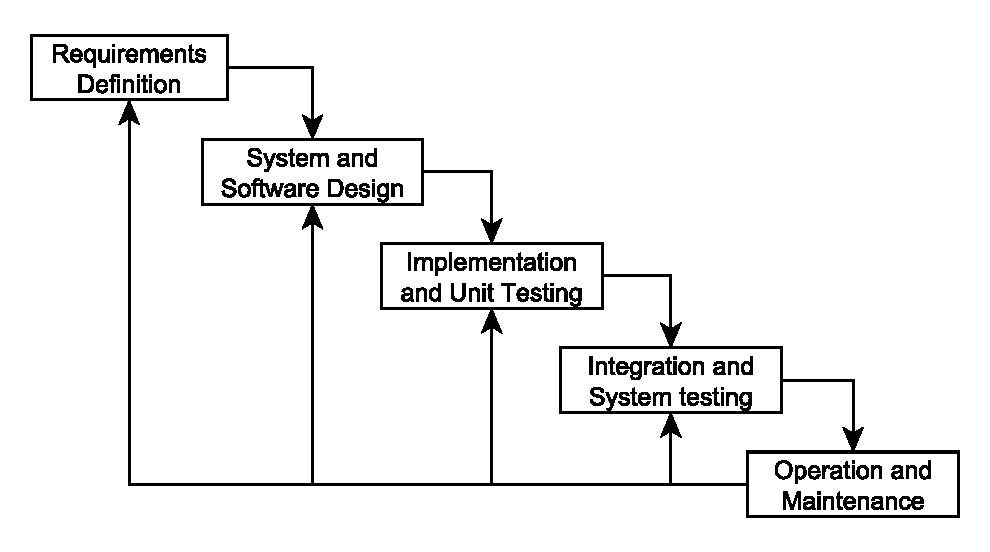
\includegraphics[width=150mm]{images/chapters/development_models/waterfall.pdf}
\caption{The Waterfall model.}
\label{waterfall}
\end{figure}

The model initially suggested by W. W. Royce discusses a linear model in which each of the aforementioned stages are used as distinct steps in the development process. Each stage is required to be completed before the next is started. This may be a sound premise in theory, but as suggested in the paper it is likely to fail in practice. The argument used is that often during development, unforeseen problems in the design are encountered. The linear model does not allow for a return to a previous stage in development. Hence, it does not allow for changes in the design that could potentially resolve such problems.

Therefore, an alternative model is suggested that allows for the process to return to earlier stages if necessary. This may not be an ideal solution either, but it does allow for encountered problems to be addressed during development.

\subsection{Agile Software Development}

As can be seen from the ending of the Waterfall-section there were doubts about its applicability already at an early stage. With the advancement of business needs and customer involvement something had to change. This opened the door for the introduction of a new software development methodology, namely agile software development. This new way of thinking tries to deal with collaboration in a way that promotes adaptive planning, early delivery and continuous improvement, making the development phase faster and more flexible regarding changes \cite{abrahamsson2002}.

\subsubsection{Scrum}
\label{scrum}

In this section an introduction to one of the most popular agile software development methodologies will be carried out, namely Scrum. This is based mainly on Abrahamsson, Salo, Ronkainen and Warsta's publication on agile methods \cite{abrahamsson2002}. In VersionOne's ``7th Annual State of Agile Development Survey'' Scrum or Scrum variants had a quoted 72\% usage making it by far the most popular agile methodology in the survey \cite{Com2013}.

Scrum is an iterative and incremental software development model (as shown in figure \ref{scrum}). It has come forth from the realisation that development methods that were common at the time of its introduction worked well in theory but did not in practice. These methods, Waterfall included, were designed to provide a structured and well-defined development process \cite{scrum}.

The agile software development processes, like Scrum, are part of a recent approach to software development. The idea with Scrum in particular is to divide the development into short periods called ``sprints''. This is done to focus effort for a limited time on short-term goals. Iterating over these goals allows the process to adapt the development plan based on progress but also to address any design problems that arise.

In short, the team concentrates on isolated parts, and through this prioritises on the most important tasks of the project first. The time span of a sprint is typically between one and four weeks long.

In order to implement the requirements step by step and in an orderly fashion, a repository is kept containing the features that have yet to be implemented. This repository is called the ``product backlog''. During development, the requirements could change over time. Therefore the product backlog is not static; it changes to the needs of the project with new topics being added, and obsolete ones being removed. The items from the backlog that a team works on during a sprint is called the ``sprint backlog''.

Meetings are also a key part of Scrum. There are several different types of meetings: sprint planning meeting, daily scrum meeting, backlog refinement, end of cycle and Scrum-of-Scrums. The sprint planning meeting is held at the beginning of each sprint cycle. Here the focus is on what work is to be done, and the sprint backlog for the coming sprint cycle is set. The daily scrum meeting, also called the daily stand-up, is a daily encounter (15 minutes) where each member of the project team answer these three questions:

\begin{enumerate}
  \item What have you done since yesterday?
  \item What are you planning to do today?
  \item Are there any impediments in your way?
\end{enumerate}

Further, there is the backlog refinement, also called ``grooming''. This is where tasks are created, large tasks are decomposed into smaller ones, tasks are prioritised, and the existing tasks are sized in the product backlog. Backlog refinement is often split into two meetings. In the first meeting the product owner and other stakeholders create and refine stories in the backlog. In the second meeting the project team sizes the tasks in the backlog to make them ready for the next sprint. Planning poker is an example of how this can be carried out.

The last listed meeting occurs at the end of each cycle, and is therefore called end of cycle (meeting). This is actually two meetings: a sprint review meeting and a sprint retrospective. At the sprint review meeting the work that is completed and yet to be finished is reviewed. The completed work is also presented for the stakeholders, often called  ``the demo''. At the sprint retrospective all members reflect on the past sprint. Two main questions are answered:

\begin{enumerate}
  \item What went well during the sprint?
  \item What could be improved in the next sprint?
\end{enumerate}

The Scrum team usually consists of five to nine members. It is important to note that Scrum teams do not use traditional roles such as programmer, tester, designer or architect. Instead the main goal for the Scrum team is to collectively complete the tasks within the sprint.

\begin{figure}[ht!]
\centering
\includegraphics[width=150mm]{images/chapters/development_models/Scrum.png}
\caption{The Scrum cycle.}
\label{scrum}
\end{figure}

To end the section, as well as making a natural shift towards the next topic (Coordination), a look at Scrum-of-Scrums is carried out. It is a natural shift because Scrum-of-Scrums are used as the coordination mechanism across teams in the Scrum methodology. It works as the daily scrums (though usually implemented on a weekly basis because of time constraints and the complexity to find common times for all teams), but with one member assigned from each Scrum team to report completions, next steps and impediments for their respective teams. It is important that these impediments focus on the challenges that may impact coordination across teams and might limit other teams' work. The Scrum-of-Scrums will have their own backlog aiming to improve the cross-team coordination \cite{Sutherland2001}. Below the suggested questions for the SoS meetings are listed \cite{Cohn2007}:

\begin{enumerate}
  \item What did your team do since the previous meeting that is relevant to some other team?
  \item What will your team do by the next meeting that is relevant to other teams?
  \item What obstacles does your team have that affect other teams or require help from them?
  \item Are you about to put something in another team's way?
\end{enumerate}

Takeuchi et al. identified three strategies for distributed Scrum teams. The first type is isolated Scrum teams where teams operate as silos and no collaboration across teams is performed violating the agile principles. The second type is Scrum-of-Scrums which means overlapping Scrum teams. Here teams coordination, communicate and collaborate across teams through SoS meetings with participants from each team involved. Lastly, totally integrated Scrum teams are suggested. In this type teams are fully distributed and each team has members located at several sites. This approach creates similar characteristics as co-location. Type B is what is most common when several Scrum teams work together. The different types are visualised in figure \ref{distributedscrum} \cite{takeuchi2004}.

\begin{figure}[ht!]
\centering
\includegraphics[width=110mm]{images/distributed_scrum.png}
\caption{Different strategies for distributed Scrum teams.}
\label{distributedscrum}
\end{figure}

\section{Coordination}

This section takes a look at different publications on coordination. It starts of with Malone and Crowston's well-known coordination theory. After this has been described a closer look at Strode's theoretical model of coordination is outlined. Ending the chapter is a brief look at the complexity factor introduced with a large-scale context in coordination.

\subsection{Malone and Crowston's Coordination Theory}

One of the most well-known papers on coordination theory was published by Malone and Crowston in 1990 and further redefined in 1994 (the focus will be on this paper) \cite{Malone1994}. Their study spans different fields and can therefore be seen as an interdisciplinary coordination study. They list an extensive amount of different definitions of coordination, and through these proposed definitions and their own work come up with a rather simple definition:

\begin{fancyquotes}
Coordination is managing dependencies between activities.
\end{fancyquotes}

These dependencies can occur when some task has to be postponed or extended because of its connection to another task, resource or unit. Their theory is based on a combination of coordination from several different disciplines such as computer science, organization theory, operations research, economics, linguistics, and psychology. They state that coordination consists of one or more coordination mechanisms, and that each of these address one or more dependencies.

While Strode et al. acknowledges their coordination theory as very useful for identifying these so-called dependencies, categorising them, and identifying coordination mechanisms in a situation, they conclude that it is only a theory for analysis and not intended to be used for prediction. Despite this being true, and the coordination theory not being suitable for predicting outcomes such as coordination effectiveness, their theory adds important information for better understanding of how activities or artefacts support coordination in organisational settings \cite{Strode2012}.

\subsection{Strode's Theoretical Model of Coordination}
\label{strodechap}

Strode et al. performed a multi-case study on three different co-located agile projects in 2012 \cite{Strode2012}. From these projects the findings led to a theoretical model of coordination that will be outlined in this section. It is important to note that these projects were not large-scale, but the model will nonetheless be used to compare if there are similarities from the model proposed by Strode et al., and the findings from the literature review on large-scale agile project coordination. This will be performed in chapter \ref{results}, \ref{disc} and \ref{concl}.

From these case studies three main components for the theoretical model were extracted: Synchronisation, Structure and Boundary Spanning. These components combine to what is called the ``Coordination Strategy''. Coordination strategy is in this context a group of coordination mechanisms that manage dependencies in a situation. The theoretical model of coordination can be seen in figure \ref{strode}. Below the three main components will be explained in more detail:

\begin{figure}
\centering
\includegraphics[width=160mm]{images/Strode.pdf}
\caption{A theory of coordination in agile software development projects.}
\label{strode}
\end{figure}

\subsubsection{Synchronisation}

Synchronisation in this context consists of synchronisation activities and synchronisation artefacts produced and used during these activities. Synchronisation activities are activities performed by all team members simultaneously. They contribute to a common understanding of the task, process, and or expertise of other team members. Synchronisation artefacts on the other hand are artefacts that are generated during synchronisation activities. These artefacts may be visible for the entire team or largely invisible but available. The artefacts can take a physical or virtual form, and are temporary or permanent.

\subsubsection{Structure}

Structure in this model is the arrangement of, and relations between, the parts of something complex. It consists of three categories: proximity, availability and substitutability. Proximity is the physical closeness of other (individual) team members. Availability means that other team members are accessible for requests or information. Lastly, substitutability has to do with the team members ability to perform others' work to maintain time schedules.

\subsubsection{Boundary Spanning}

The last component of the coordination strategy is boundary spanning. Boundary spanning has to do with the interaction with other organisations or other business units that are not involved in the project. It consists of three aspects: boundary spanning activities, boundary spanning artefacts and a coordinator role. Boundary spanning activities are activities performed to achieve help from some unit or organisation not involved in the project. The boundary spanning artefacts are artefacts produced to enable this external coordination. These artefacts have the same characteristics as synchronisation artefacts. Lastly, the coordinator role is a role taken by someone within the project team. His or her role is to support interaction to outside personnel to extract resources or information needed in the project at hand.

\subsubsection{Coordination Effectiveness}

There is another important part of the theoretical model of coordination, namely the coordination effectiveness concept. This concept will be further explained in section \ref{efficiency} that takes a look at coordination effectiveness.

\subsubsection{Propositions}

There are in total ten propositions (Proposition 1 has two parts) linking the coordination concepts in Strode's theoretical coordination model showed in figure \ref{strode}. These are outlined below:

\begin{fancyquotes}
\textbf{Proposition 1a:} A coordination strategy that includes synchronisation and structure coordination mechanisms improves project coordination effectiveness when the customer is included in the project team. Synchronisation activities and associated artefacts are required at all frequencies – project, iteration, daily, and ad hoc.
\end{fancyquotes}

\begin{fancyquotes}
\textbf{Proposition 1b:} A coordination strategy that includes synchronisation, structure, and boundary spanning coordination mechanisms improves project coordination effectiveness when the customer is an external party to the project. Synchronisation activities and associated artefacts are required at all frequencies – project, iteration, daily, and ad hoc. Boundary spanning activities and associated artefacts are required at all frequencies – project, iteration, and ad hoc.
\end{fancyquotes}

\begin{fancyquotes}
\textbf{Proposition 2:} Synchronisation activities at all frequencies – project, iteration, daily, and ad hoc, along with their associated synchronisation artefacts, increase implicit coordination effectiveness.
\end{fancyquotes}

\begin{fancyquotes}
\textbf{Proposition 3:} Structural coordination mechanisms i.e. close proximity, high availability, and high substitutability, increase implicit coordination effectiveness.
\end{fancyquotes}

\begin{fancyquotes}
\textbf{Proposition 4:} High levels of boundary spanning coordination mechanisms, i.e. boundary spanning activities at all frequencies – project, iteration, and ad hoc, their associated boundary spanning artefacts, and a coordinator role, increases explicit coordination effectiveness.
\end{fancyquotes}

\begin{fancyquotes}
\textbf{Proposition 5:} Under conditions of high project complexity, increasing the frequency of iteration and ad hoc synchronisation activities will maintain coordination effectiveness. The production of related synchronisation artefacts must be adjusted accordingly.
\end{fancyquotes}

\begin{fancyquotes}
\textbf{Proposition 6:} Under conditions of high project uncertainty, to maintain synchronisation activity frequency and production of associated artefacts, changing the priority of stories will maintain coordination effectiveness.
\end{fancyquotes}

\begin{fancyquotes}
\textbf{Proposition 7:} A mono-project organisation structure enables close proximity relative to multi- or matrix structures.
\end{fancyquotes}

\begin{fancyquotes}
\textbf{Proposition 8:} A mono-project organisation structure improves availability relative to multi- or matrix style structures.
\end{fancyquotes}

\begin{fancyquotes}
\textbf{Proposition 9:} Under conditions of high project uncertainty, when the customer is not part of the team, increased boundary spanning coordination mechanisms will maintain coordination effectiveness. The production of related boundary spanning artefacts must be adjusted accordingly.
\end{fancyquotes}

\subsection{Coordination in Large-scale}
\label{largescalecor}

This section takes a closer look at general studies performed on large-scale coordination and is not specifically focusing on software development. The section is added to highlight the introduction of complexity that a large-scale context brings with it.

Van der Ven et al. released an article in 1976 where they tried to identify determinants of coordination modes within organisations. They state that an increase in size will produce a trade-off between the increasing complexity and cost of coordination at the administrative level. From the research two different coordination forms are described, namely vertical and horizontal. The vertical communication includes coordination through curators, while the horizontal communication occurs by way of one-to-one communication. Their findings show that when team size increases the coordination moves towards a more vertical and impersonal style \cite{Ven1976}. This is backed up by John Child in a publication from 1973. Here he states that with a growing complexity level there is likely that administrative problems will occur regarding coordination and control \cite{Child1973}.

\section{Large-scale}

Having looked at coordination in large-scale in section \ref{largescalecor}, what is actually this so-called ``large-scale''? This was a topic brought up at a workshop regarding research challenges in large-scale agile software development where opinions regarding how large-scale should be defined varied a lot. Some suggestions were to define it through project duration, project cost, number of people involved, number of remote sites and/or number of teams \cite{Dingsoyr2013b}. This issue was further analysed by Dingsøyr, Fægri and Itkonen trying to work out a taxonomy of scale for agile software development. Their results are summarised in table \ref{Scale} where the taxonomy of scale is based on the amount of teams involved in the development project \cite{Dingsoyr2013a}.

\begin{table}[H]
\begin{center}
    \begin{tabular}{| l | l | p{7cm} |}
    \hline
    \textbf{Level} & \textbf{Number of teams} & \textbf{Coordination approaches} \\ \hline
    Small-scale & 1 & Coordinating the team can be done using agile practices such as daily meetings, common planning, review and retrospective meetings. \\ \hline
    Large-scale & 2-9 & Coordination of teams can be achieved in a new forum such as a Scrum of Scrums forum. \\ \hline
    Very large-scale & 10+ & Several forums are needed for coordination, such as multiple Scrum of Scrums. \\
    \hline
    \end{tabular}
    \caption{A taxonomy of scale of agile software development projects.}
    \label{Scale}
\end{center}
\end{table}

Others have also discussed problems regarding large-scale. For example Schnitter and Mackert discuss the scaling of Scrum at SAP AG and concludes that in their case the maximum involved development employees that may be organised with regards to agile project management is 130 (This number sums up developers in 7 teams (max. 70 people), the product team (max. 16), development infrastructure responsible (about 10), quality assurance and testers (about 25), general management (about 10)) \cite{Nord2011}.

Another example is taken from Nord et al. defining large-scale by scope of the system, team size, and project duration. They say that the size of the development team must be more than 18 people and distributed into a few teams \cite{Robert2014}.

So the definition of a ``large-scale agile project'' used in this research will be:

\begin{fancyquotes}
An agile project must consist of a minimum amount of two teams coordinating across the teams to be categorised as large-scale.
\end{fancyquotes}

\section{Efficiency, Effectiveness, Productivity and Performance in Coordination}
\label{efficiency}

There has been released a good amount of papers regarding effectiveness, productivity and efficiency in project literature. Unfortunately research in this area that focuses on large-scale is scarce. Therefore, the work highlighted in this section will mainly be extracted from small-scale studies. To start the section of a closer look at the aforementioned study by Strode et al. will be performed, before a summary of some different field studies on the matter will be carried out.

\subsection{Strode's Coordination Effectiveness}
\label{cordinationeffectiveness}

Part of the theoretical model of coordination by Strode et al. seen in figure \ref{strode} is the so-called ``coordination effectiveness''. This concept was developed by Strode et al. in 2011 having used the same three agile projects discussed earlier, as well as a non-agile software development project as a foundation \cite{Strode2011}. Coordination effectiveness is defined as the outcome of a particular coordination strategy. Coordination effectiveness is split into two components: an implicit and an explicit part.

The implicit part is concerned with coordination that occurs without explicit speech or message passing, this happens within work groups. It has five components: ``Know why'', ``Know what is going on and when'', ``Know what to do and when'', ``Know who is doing what'', and ``Know who knows what''. These aspects are pretty self-explanatory.

The explicit component on the other hand is concerned with the physical aspects of the project. It states that the objects involved in the project have to be in the correct place, at the correct time and in a state of readiness for use. A summary of the combination of explicit and implicit coordination effectiveness is provided in figure \ref{effectiveness}.

\begin{figure}[H]
\centering
\includegraphics[trim=0cm 17.5cm 0cm 1.5cm, width=160mm]{images/Coordination_Effectiveness.pdf}
\caption{Components of coordination effectiveness from Strode et al. (2011).}
\label{effectiveness}
\end{figure}

To end this subsection a definition of coordination effectiveness from Strode et al. is provided:

\begin{fancyquotes}
Coordination effectiveness is a state of coordination wherein the entire agile software development team has a comprehensive understanding of the project goal, the project priorities, what is going on and when, what they as individuals need to do and when, who is doing what, and how each individuals work fits in with other team members work. In addition, every object (thing or resource) needed to meet a project goal is in the correct place or location at the correct time and in a state of readiness for use from the perspective of each individual involved in the project \cite{Strode2011}.
\end{fancyquotes}

\subsection{Some Studies on the Field}

Below four studies that try to identify important factors of coordination's impact on team performance are described.

\subsubsection{Team Effectiveness 1997-2007: A Review of Recent Advancements and a Glimpse Into the Future}

Mathieu et al. takes a look at literature published on team effectiveness in a ten year period. They look at several different aspects regarding the nature of teamwork \cite{Mathieu2008}. It is important to note that the main focus of this article is on small-scale teams, and that the publications used are not gathered directly from the software and agile field. However, the article gives perspectives that are noteworthy. The main focal point here will be on Mathieu's chapter on organisational contexts, and the section on multi-team systems coordination in particular.

One aspect that was identified in several studies having a positive impact on performance was an ``openness climate''. What was concluded at the macro organisational level was that a support for a openness climate at the broader level of the organisation had a positive impact on team level processes.

Quite a few studies were identified on multi-team systems coordination as well. Here, the findings showed a positive correlation between inter-team coordination and intra-team coordination. Hyatt et al. indicated that teams perform more effectively as self-contained units when they have robust information networks, as well as communication and cooperation channels, both within and between teams \cite{Hyatt1997}. This again highlights the importance of studies focusing on coordination in large-scale.

\subsubsection{Interpretative Case Studies on Agile Team Productivity and Management}

Melo et al. performed a multi-case study on three large Brazilian IT companies that were using agile methods in their projects \cite{Melo2013}. The objective of the research was to provide a better understanding of which factors that had an impact on agile team productivity. To document teamwork effectiveness they used the well-known theoretical model ``Input-Process-Outcome'' (IPO). Their input factors were ``Individual and Group characteristics'', ``Stage of team development'', ``Nature of task'', ``Organizational context'' and ``Supervisory behaviors''. One process-category was identified: ``Group processes''. Lastly they identified two outcome-groups, namely ``Agile team productivity'' and ``Attitudinal and Behavioral''. All of these are summarised constituting the conceptual framework for their agile team productivity in figure \ref{atpcf}.

\begin{figure}[ht!]
\centering
\includegraphics[width=150mm]{images/IPO.png}
\caption{Agile team productivity conceptual framework.}
\label{atpcf}
\end{figure}

After collecting the data from their multi-case study they mapped the results in a thematic map on agile productivity factors. These findings showed three main groups of team management and their impact on productivity. For this study it is the ``Inter-team coordination'' and ``Team design choices'' that are interesting because of their impact on coordination to a larger degree, meaning ``Team member turnover'' is left out. 

In ``Team design choices'' four roots of impact were identified: ``Team size'', ``Team members skills'', ``Team collocation'' and ``Team members allocation''. Out of these team collocation and team size seem to effect coordination effectiveness the most. Their findings showed that smaller teams led to better communication and alignment, while collocation had a positive influence on team productivity as it helped overcome invisible barriers between teams in a hierarchical company.

For ``Inter-team coordination'' two roots were identified: ``Lack of commitment among teams'' and ``Inappropriate coordination rules among teams''. One of the main reasons for negative impact was identified to be external dependencies because projects often were left waiting for results of entities outside the project team. So a problem in inter-team coordination was misalignment, hence, synchronisation is an important factor.

\subsubsection{Dispersion, Coordination and Performance in Global Software Teams: A Systematic Review}

Anh et al. performed a systematic literature review (SLR) to collect relevant studies on dispersion, coordination and performance in global software development (GSD), and highlighted the findings of impact factors in a thematic mapping \cite{Anh2012}. It is important to note that the findings are not from agile software development, but they are still interesting because of the global aspect in the literature used. The results are briefly summarised in table \ref{GSD}:

\begin{table}[H]
\begin{center}
    \begin{tabular}{ | p{5cm} | p{8cm} |}
    \hline
    \textbf{Type} & \textbf{Impact on team performance} \\ \hline
    Presence of geographical dispersion & Negative (work takes longer time, less effective communication and coordination) \\ \hline
    Number of sites/Team size & Negative (complicates coordination and hampers communication) \\ \hline
    Large time zone differences between teams & Negative (creates coordination problems because of the complexity introduced) \\ \hline
    \end{tabular}
    \caption{Impact of geographical dispersion on performance.}
    \label{GSD}
\end{center}
\end{table}

\subsubsection{Team Performance in Agile Development Teams: Findings from 18 Focus Groups}

Dingsøyr and Lindsjørn carried out a focus group study looking at which factors the agile software practitioners in the research perceived as influential on effective teamwork \cite{Dingsoyr2013c}. This paper focuses on the team performance of individual teams, but is included because of its agile nature. To place the suggestions from the participants into categorise Dingsøyr et al. decided to use the ``Big Five'' model proposed by Salas et al. \cite{Salas2005} leading to eight teamwork components: ``Team leadership'', ``Mutual performance monitoring'', ``Backup behaviour'', ``Adaptability'', ``Team orientation'', ``Shared mental models'', ``Mutual trust'' and ``Closed-loop communication''. A summary of the distribution of all suggestions over these components is outlined in table \ref{summary2}.

\begin{table}[H]
\begin{center}
    \begin{tabular}{ | p{6cm} | p{2.5cm} | p{2.5cm} | p{2.5cm} |}
    \hline
    \textbf{Teamwork component} & \textbf{Foster} & \textbf{Hinder} & \textbf{Total} \\ \hline
    Team leadership & 90 & 139 & 229 \\ \hline
    Mutual performance monitoring & 49 & 22 & 71 \\ \hline
    Backup behaviour & 44 & 57 & 101 \\ \hline
    Adaptability & 46 & 50 & 96 \\ \hline
    Team orientation & 91 & 65 & 156 \\ \hline
    Shared mental models & 104 & 59 & 163 \\ \hline
    Mutual trust & 97 & 58 & 155 \\ \hline
    Closed-loop communication & 122 & 90 & 212 \\ \hline
    Sum & 643 & 540 & 1183 \\ \hline
    \end{tabular}
    \caption{Summary of the distribution of suggestions over teamwork components.}
    \label{summary2}
\end{center}
\end{table}

The teamwork component with the strongest connection to coordination is ``closed-loop communication''. Looking at table \ref{summary2} a lot of emphasis was aimed towards the component from the practitioners (second highest total count). This again illustrates the importance of coordination. The sub-components identified of closed-loop communication are outlined in table \ref{closedloop}.

\begin{table}[H]
\begin{center}
    \begin{tabular}{ | p{4cm} | p{5.25cm} | p{5.25cm} |}
    \hline
    \textbf{Sub-component} & \textbf{Foster} & \textbf{Hinder} \\ \hline
    Co-location & Physical presence \newline Co-location \newline Physically placed together & People are distributed \newline Distance \newline Not co-located \\ \hline
    Openness & Open communication \newline Openness in the team \newline Open dialogue & Secrecy \newline Retaining information \\ \hline
    Infrastructure & Process support tools \newline Suitable office spaces \newline Tools that work & Bad tools \newline Bad office facilities \\ \hline
    Visualising status and progress & Informative workspace \newline Visualise things that go well \newline Whiteboard/task-board & No whiteboards \\ \hline
    Social atmosphere & Good atmosphere \newline Fun \newline Friendly tone & Scolding \newline Antisocial environment \newline Bad atmosphere \\ \hline
    \end{tabular}
    \caption{Sub-components identified of closed-loop communication with their respective performance items.}
    \label{closedloop}
\end{center}
\end{table}

As can be seen from table \ref{closedloop} a lot of attention was directed towards location of team members, infrastructure and supportive tools, and organisational culture. The presence of co-location, a good infrastructure and supportive tools, and an open and social climate seem to all have a positive effect on team effectiveness.

\subsubsection{Summary}

The findings from the different studies are summarised in table \ref{summary}. Note that it could be argued that misalignment and synchronisation, as well as team collocation and presence of geographical dispersion, are contrasts of each other. They are however included in the summary table because they were identified as important aspects in the different studies.

\begin{table}[H]
\begin{center}
    \begin{tabular}{ | p{8cm} | p{6cm} |}
    \hline
    \textbf{Type} & \textbf{Impact} \\ \hline
    Organisational openness culture & \textcolor{ForestGreen}{Positive} \\ \hline
    Misalignment & \textcolor{red}{Negative} \\ \hline
    Synchronisation & \textcolor{ForestGreen}{Positive} \\ \hline
    Team co-location & \textcolor{ForestGreen}{Positive} \\ \hline
    Presence of geographical dispersion & \textcolor{red}{Negative} \\ \hline
    Number of sites/Team size & \textcolor{red}{Negative} \\ \hline
    Large time zone differences between teams & \textcolor{red}{Negative} \\ \hline
    Infrastructure/Supportive tools & \textcolor{ForestGreen}{Positive} \\ \hline
    \end{tabular}
    \caption{Summary of impacts identified in the studies.}
    \label{summary}
\end{center}
\end{table}
\chapter{Method}

\minitoc

The research study used different methods to gather relevant publications and theory. These are further outlined in this chapter starting with a detailed look at the literature review performed, as well as highlighting other parts of the gathering methodology, namely snowball sampling and general accumulation of papers. After this has been performed the research method is outlined in more detail. The focus here will be on ``case selection'', ``data collection'' and ``data analysis''.

\newpage

\section{Literature Review}

For this study a literature review was chosen as one of the information gathering methods. For the searching process and selection of articles in the literature review certain recommendations from systematic reviews were followed. The general procedure of such a review is outlined in L1 below. It is important to note that the searching had an open-mindedness regarding search words and the selection process.

\vspace{0.5cm}

\begin{tcolorbox}[breakable, enhanced]
%\fbox{\parbox{\textwidth}{L1 - The steps of a systematic review \cite{khan2003}:
\textbf{L1 - The steps of a systematic review \cite{khan2003}:}

\begin{enumerate}
  \item Framing questions for a review.
  \item Identifying relevant work.
  \item Assessing the quality of studies.
  \item Summarizing the evidence.
  \item Interpreting the findings.
\end{enumerate}
\end{tcolorbox}

\vspace{0.5cm}

Some of the benefits and objectives of a literature review are summarised in L2 below.

\vspace{0.5cm}

\begin{tcolorbox}[breakable, enhanced]
%\fbox{\parbox{\textwidth}{L2 - Objectives of a literature review \cite{Oates2006}:
\textbf{L2 - Objectives of a literature review \cite{Oates2006}:}

\begin{itemize}
  \item Show that the researcher is aware of existing work in the chosen topic area.
  \item Place the researcher's work in the context of what has already been published.
  \item Point to strengths, weaknesses, omissions or bias in the previous work.
  \item Identify key issues or crucial questions that are troubling the research community.
  \item Point to gaps that have not previously been identified or addressed by researchers.
  \item Identify theories that the researcher will test or explore by gathering data from the field.
  \item Suggest theories that might explain data the researcher has gathered from the field.
  \item Identify theories, genres, methods or algorithms that will be incorporated in the development of a computer application.
  \item Identify research methods or strategies that the researcher will use in the research.
  \item Enable subsequent researchers to understand the field and the researcher's work within that field.
\end{itemize}
\end{tcolorbox}

\vspace{0.5cm}

\subsection{General Outline}

As explained in subsection \ref{general} a set of articles and publications were provided by the supervisor to give an overview on the field and agile software development in general. This made it easier to classify which studies to look for and how to evaluate their relevance and rigour. The databases used in the literature review are summarised in table \ref{databases}. When searching in these databases concepts and keywords were combined to match the research question as well as other interesting combinations. These concepts and keywords are outlined in table \ref{searchwords}. It is important to note that the last concept was additional search words used because of their close relation to coordination and team performance.

\begin{table}[H]
\begin{center}
    \begin{tabular}{ | p{4cm} | p{7.5cm} |}
    \hline
    \textbf{Name} & \textbf{Impact} \\ \hline
    ISI Web of Science & apps.webofknowledge.com \\ \hline
    ACM Digital Library & dl.acm.org  \\ \hline
    Science Direct (Elsevier) & sciencedirect.com \\ \hline
    Google Scholar & scholar.google.com \\ \hline
    \end{tabular}
    \caption{Databases used in the literature review.}
    \label{databases}
\end{center}
\end{table}

%\begin{table}[H]
\begin{center}
    \begin{longtable}{ | p{4cm} | p{7.5cm} |}

    \hline \textbf{Concept} & \textbf{Keywords} \\ \hline
    \endfirsthead

    \multicolumn{2}{c}%
{{\bfseries \tablename\ \thetable{} -- continued from previous page}} \\ \hline
    \textbf{Concept} & \textbf{Keywords} \\ \hline
    \endhead

    \multicolumn{2}{|r|}{{Continued on the next page\ldots}} \\ \hline
    \endfoot

   \endlastfoot

    Coordination & Communication, Collaboration, Inter-team coordination, Closed-loop communication \\ \hline
    Agile & Scrum, XP, Crystal, Lean, Kanban, Scrumban, Scrum ban, Scrum-ban, Extreme Programming, Xtreme Programming, Pair programming, Pair-programming  \\ \hline
    Large-scale & Global, Multiteam systems, Multi-team systems, MTS, Multi-agent systems, Distributed, International \\ \hline
    Effectiveness & Efficiency, Productivity, Performance \\ \hline
    Additional search words & Co-located, Collocated, Colocated, Co located, Distributed, Dispersed, Global, Globally, International, Mental model, Team mental model, Shared mental model, Strategic mental model, Trust, Mutual trust \\ \hline
    \caption{Search words used in the literature review.}
    \label{searchwords}
    \end{longtable}
\end{center}
%\end{table}

The literature review provided an extensive amount of findings, unfortunately a lot of the publications were focusing on small-scale development. Therefore, a selection process had to be carried out. Here all abstracts of the collected literature were read and publications with the highest relevance were chosen. The articles that were still left after this selection process were then read thoroughly where some were discarded to give an appropriate amount of publications. The analysis outlined above focused mainly on finding articles focusing on large-scale agile inter-team coordination, meaning such articles were given a higher score when identified. Some other aspects that contributed to the score were mentioning of global projects, effectiveness and inter-team coordination in general. This process was important because of the time constraints specified on the study, and to obtain relevant and rigorous literature to insure a robust study.

\subsection{Snowball Sampling}

Snowball sampling is a term that reflects how new studies are selected through already chosen studies (based on their similarities) \cite{Goodman1961}. This was done in two ways in the research. In table \ref{databases} a list of databases used for the literature review are summarised. Some of these databases provided snowball sampling in the way of suggesting similar articles when a specific publication was selected from a search. This is the first way of snowballing used. The second way was through using reference lists in selected articles and publications. This extraction lead to a lot of well-written and recognised papers.

\subsection{General Accumulation}
\label{general}

Articles were also accumulated through a supervisor and fellow research students. At the start a handful of publications were received from the supervisor, and other papers were also acquired throughout the study. It is important to note that all the articles were inspected in the same manner as the publications found from the literature review to make sure their relevance and rigour were appropriate.

\section{Research Method}

Because there has been few studies on the field of inter-team coordination in large-scale agile software development an exploratory case study was chosen as the research method. An exploratory case study is an excellent fit to get a greater understanding of somewhat unexplored territories, as well as spawning possibilities for further research. Details about exploratory case studies is further outlined in the quotation below.

\begin{fancyquotes}
An exploratory study is used to define the questions or hypotheses to be used in a subsequent study. It is used to help a researcher understand a research problem. It might be used, for example, where there is little in the literature about a topic, so a real-life instance is investigated, in order to identify the topics to be covered in a subsequent research project \cite{yin2009case}. 
\end{fancyquotes}

To choose an appropriate case organisation and project certain criteria had to be present. These are further discussed in section \ref{case_selection}. In the end one case was selected as the focus because of its availability, as well as the case successfully fulfilling the case criteria. The case was described as the most successful large-scale agile software development project in Norway so far. The project will be referred to as ``Omega'' throughout this thesis and was a project to develop a new office automation system for the public department ``Gamma''. The Omega-project ran from 2008 to 2012, and had at most 13 development teams involved. The distribution of these teams were six Gamma-teams, as well as four Alfa-teams and three Beta-teams. ``Alfa'' and ``Beta'' were contracted consulting companies in the Omega-project. The project as a whole is outlined in more detail in chapter \ref{results}.

Data collection was granted by all three organisations. Before the data collection took place it was important to get a better overview of the project and case at hand. Therefore available data was looked at in detail, e.g., public presentations. Because of this early review the complexity level of the Omega-project was identified at the initiating stages of the case study with a total of 175 people being involved in the project and sub-projects. As a result of the data collection starting some time after the project had ended a few challenges had to be dealt with, e.g., personnel availability and possible holes in memories of participants.

\subsection{Case Selection}
\label{case_selection}

Before the case study was conducted several criteria for a fitting case project were agreed upon. Seeing as the research was suppose to focus on large-scale development/multi-team systems it was important to find a case where minimum two teams were present in the project, as well as collaborating across the teams. It was also important that the project performed in the case was an agile software development project. Another criteria was that the length of the project had to be suitable, meaning that the project had been ongoing for a reasonable amount of time. The reasoning behind this was that the amount of data would be richer, and it would be easier to find patterns over a longer period of time.

There were also other criteria which were preferable, but not mandatory. One of these criteria was that it would be desirable if there were several roles within the project as a whole and the project teams. This had to do with the possibility of people with different roles within a project having various experiences from the course of the project leading to valuable data, or put in other words, having different points of view within the project. Another preferred criteria was having a large-scale project with several organisations involved. With several organisations involved there will be different cultures and protocols involved, and therefore a lot of interesting data could surface when comparing the approach of the different organisations.

\subsection{Data Collection}

For the data collection in the exploratory case study focus groups were selected. In these focus groups aspects that are known to be challenging in large-scale agile software development were brought up, as well as general discussion on the topics of large-scale software development, inter-team coordination and team performance. Focus groups are further outlined in L3, and were primarily selected because of their ability to accumulate extensive and valuable amounts of research data.

In total three focus groups were conducted, one for each of the organisations involved. The topic that was looked at in the focus groups was ``Inter-team coordination and knowledge sharing''. The reasoning behind conducting focus groups for each of the organisations, and not performing them on a project level, was to make sure that an openness was achieved, and that data concerning specific organisations were not lost. As mentioned in section \ref{case_selection} there might be differences in cultures and methodologies between organisations, and these might not have been present in the focus groups if they were held on a joint basis.

The organisations were asked to provide their most relevant personnel to attend each focus group. In total 8 participants were involved in the focus groups. The participants had several roles in the Omega-project: development managers, scrum masters, (sub-)project managers, developers, delivery managers, functional architects and technical architects. It is important to note that most of the focus group participants were employees in management positions in the project. Most of these participants started as developers before switching to management roles through the course of the project. Because of the availability of personnel and topic in the focus groups no pure developers were present. The distribution of participants in the different focus groups is summarised in table \ref{pifg}.

\begin{table}[H]
\begin{center}
    \begin{tabular}{ | p{5cm} | p{3cm} | p{3cm} |}
    \hline
    \textbf{Theme} & \textbf{Organisation} & \textbf{Number of participants} \\ \hline
    \multirow{3}{*}{} & Alpha & 2 \\ \cline{2-3}
    Inter-team coordination and knowledge sharing & Beta & 3 \\ \cline{2-3}
    & Gamma & 3 \\ \hline
    \end{tabular}
    \caption{Participants in focus groups.}
    \label{pifg}
\end{center}
\end{table}

Before the focus group sessions were conducted interview guides were developed (these can be seen in appendix \ref{interview_guide}), as well as a rough timeline of the project. The timeline was used to freshen the participants' memories about key events. In the focus groups the role of the researcher was to moderate the discussion and take notes. At the start of each focus group the participants were asked to explain their role(s) in the Omega-project. All of the focus group meetings were recorded digitally and transcribed at a later point in time, and whiteboard drawings were documented through pictures. In total the three focus groups resulted in 94 pages of transcribed material. Minutes of each focus group was also sent to each of the corresponding participants for needed information and review.

\newpage

\begin{tcolorbox}[breakable, enhanced]
%\fbox{\parbox{\textwidth}{L3 -  Focus group \cite{Kitzinger2005}:
\textbf{L3 -  Focus group \cite{Kitzinger2005}:}

\vspace{0.5cm}

\begin{fancyquotes}
Focus groups are a form of group interview that capitalises on communication between research participants in order to generate data. Although group interviews are often used simply as a quick and convenient way to collect data from several people simultaneously, focus groups explicitly use group interaction as part of the method. This means that instead of the researcher asking each person to respond to a question in turn, people are encouraged to talk to one another: asking questions, exchanging anecdotes and commenting on each others' experiences and points of views. The method is particularly useful for exploring people's knowledge and experiences and can be used to examine not only what people think but how they think and why they think that way.
\end{fancyquotes}

\vspace{0.5cm}

The interaction in focus groups can be used to achieve seven main goals:

\begin{itemize}
  \item To highlight the respondents' attitudes, priorities, language, and framework of understanding;
  \item To encourage research participants to generate and explore their own questions and develop their own analysis of common experiences;
  \item To encourage a variety of communication from participants, tapping into a wide range and form of understanding;
  \item To help to identify group norms and cultural values;
  \item To provide insight into the operation of group social processes in the articulation of knowledge (for example, through the examination of what information is censured or muted within the group);
  \item To encourage open conversation about embarrassing subjects and to permit the expression of criticism;
  \item Generally to facilitate the expression of ideas and experiences that might be left underdeveloped in an interview and to illuminate the research participants' perspectives through the debate within the group.
\end{itemize}
%}}
\end{tcolorbox}

\vspace{0.5cm}

\subsection{Data Analysis}

After all the research data from the data collection phase was transcribed the data analysis could commence. An important aspect in qualitative data analysis is abstracting the research data to themes and patterns important to the research topic. Several steps were taken to find these themes and patterns. To start of the data analysis the 94 pages of transcribed material were read through twice to get a general overview of the data. After this was done a more thorough read-through was performed where the text was segmented into different themes, e.g., roles, methodologies and general descriptive information. Some of the themes that were identified were then further examined because of their relevance towards the research topic.
\chapter{Results}
\label{results}

\minitoc

In this chapter relevant articles gathered on ...

\newpage

\section{Introduction and Clarification}

\begin{table}[H]
\begin{center}
    \begin{tabular}{| p{5cm} | p{3.7cm} | p{1cm} | p{4cm} |}
    \hline
    \textbf{Article Name} & \textbf{Author(s)} & \textbf{Year} & \textbf{Keywords} \\ \hline
    Inter-team Coordination in Large-scale Globally Distributed Scrum: Do Scrum-of-Scrums Really Work? & Maria Paasivaara, Casper Lassenius, Ville T. Heikkilä & 2012 & Agile Software Development; Distributed Scrum; Global Software Engineering; Inter-team Coordination \\ \hline
    Communities of Practice in a Large Distributed Agile Software Development Organization – Case Ericsson & Maria Paasivaara, Casper Lassenius & 2014 & Communities of Practice; Large-scale Agile Software Development; Scaling Agile \\ \hline
    Operational Release Planning in Large-scale Scrum with Multiple Stakeholders – A Longitudinal Case Study at F-Secure Corporation & Ville T. Heikkilä, Maria Paasivaara, Kristian Rautiainen, Casper Lassenius, Towo Toivola, Janne Järvinen & 2015 & Agile Software Development; Scrum; Large Projects; Release Planning; Software Project Management \\ \hline
Towards a Governance Framework for Chains of Scrum Teams & Jan Vlietland, Hans van Vliet & 2015 & Agile; Chain of Scrum Teams; Coordination; Priority; Alignment; Predictability \\ \hline
    \end{tabular}
    \caption{Summary of articles used in this chapter.}
    \label{soauitc}
\end{center}
\end{table}

\begin{table}[H]
\begin{center}
    \begin{tabular}{| p{4cm} | p{8cm} |}
    \hline
    \textbf{Role} & \textbf{Description of role} \\ \hline
    Scrum master & \\ \hline
    Functional architect & \\ \hline
    Technical architect & \\ \hline
    Tester & \\ \hline
    Developer & \\ \hline
    \end{tabular}
    \caption{Team roles present in Scrum teams.}
    \label{trpist}
\end{center}
\end{table}

\begin{figure}[H]
\centering
\includegraphics[trim = 40mm 0mm 7mm 0mm,width=180mm]{images/omega_organisation.png}
\caption{Omega-project's organisation.}
\label{omega}
\end{figure}

\begin{figure}[H]
\centering
\includegraphics[angle=90, trim = 0mm 0mm 20mm 0mm,width=160mm, height=230mm]{images/execution_model.png}
\caption{Project execution model.}
\label{project_execution}
\end{figure}

\begin{figure}[H]
\centering
\includegraphics[angle=90, trim = 0mm 0mm 20mm 0mm,width=160mm, height=230mm]{images/initial_development_process}
\caption{Initial development process.}
\label{initial_development_process}
\end{figure}

%\begin{table}[H]
\begin{center}
    \begin{longtable}{| p{6cm} | p{9cm} |}

    \hline \textbf{Coordination mechanism} & \textbf{Description of mechanism} \\ \hline
    \endfirsthead

    \multicolumn{2}{c}%
{{\bfseries \tablename\ \thetable{} -- continued from previous page}} \\ \hline
    \textbf{Coordination mechanism} & \textbf{Description of mechanism} \\ \hline
    \endhead

    \multicolumn{2}{|r|}{{Continued on the next page\ldots}} \\ \hline
    \endfoot

   \endlastfoot

    Metascrum & A meeting similar to Scrum of Scrums but with less details which was held twice per week. Attending the metascrum was the project leaders and all the sub-project leaders from test, architecture, business and development. A ``technical metascrum'' was tried, but was shortly shut down after initiation. \\ \hline
    Planning day & The planning day was a form of kick-off for each sprint iteration where the project members met up with the project owner. The planning day was performed on three levels: project, organisation (Alpha, Beta and Gamma) and team. A rough sketch of the focus areas and work to be performed in the coming sprint was presented with a distribution towards each of the three organisations by the project owner. After this the organisations distributed the work on their respective teams, and lastly the teams got together separately and worked out a contract with estimated work to be performed which was delivered to the project owner team. Before the planning day commenced the developers also had a ``developer forum'' where development-oriented information and discussion was carried out. This was however held on an organisation basis, and not across the three organisations. \\ \hline
    Demo & Demo presentations were held by all Scrum teams at the end of each sprint iteration where everyone could attend. Each team was allocated approximately 10 minutes. There were also larger demo presentations for the project owner when a new release was finished. Some teams in addition started performing smaller demo sessions within the iterations to get rapid feedback. \\ \hline
    Pre-planning day & Before the ``planning day'' was carried out a pre-planning day was performed. Here typically different types of architects (especially functional architects) and the project owner (as well as some other members of the project owner's team) met to create a rough classification and allocation of work to the different Scrum teams for the coming sprint iteration. The allocated work was listed in a prioritised manner. \\ \hline
    Dependency meeting & A meeting held between all Scrum masters from the Alpha, Beta and Gamma teams. This meeting was held on the ``Planning day'' where the focus was on discovering dependencies across Scrum teams. However, these meetings faded away early on because of the dependencies being discovered and handled elsewhere. \\ \hline
    Solution description / ``Master plan'' & At the start of the Omega-project a larger solution description phase was performed involving a lot of architects (as can be seen from figure \ref{project_execution}). This lead to a ``master plan'' for the project and was documented in an issue tracker program called Jira. The ``master plan'' was continuously altered throughout the course of the development phase as outlined in figure \ref{initial_development_process}. In the solution description meetings important aspects were discussed such as coordination across organisations and management of activities. An example of what came out of these meetings was a dependency map of the whole Omega-project, which was in constant change. Part of the solution description meetings were also negotiation and estimation meetings which were important for the contract for each release. \\ \hline
    Jira and Wiki/Confluence & Different programs and forums were used for documentation and tracking within the project. In Jira all user stories and epics were located, and different information about the project and current sprint iteration could be seen on different levels, such as project and team level. The dependency map for the whole Omega-project was also located in Jira. Confluence was the main program used as a wiki. Here solution descriptions, team routines, routines across teams, system documentation, check lists, retrospectives, architectural guidelines, functional test etc. were all located. \\ \hline
    Open-space & An arena held on a voluntary and need basis, which was used for exchanging experiences. Only used during a few of the releases. Participants suggested the topics beforehand, leading to agendas for open-space sessions. \\ \hline
    Jabber & Jabber was introduced as an instant messaging service in the Omega-project after being identified as something needed in one of the Open-space sessions. Project members could ask both formal questions, e.g., technical questions, and informal questions or activities, e.g., wine lotteries. \\ \hline
    Lunch seminars & Kind of similar to the ``open-space'' sessions. Typically two to three topics were held by project-personnel on relevant and interesting topics, often regarding themes correlated to the current situation of the project. As with the ``open-space'' session these seminars were also held on a certain period of the project before fading away. \\ \hline
    Front-end meeting & The front-end developers worked with a complex framework called Flex. Because of this a lot of coordination had to be handled between teams working with this framework from all organisations. Therefore, front-end meetings where held were typically the most prominent Flex-developers were present. \\ \hline
    Technical architecture forum & At the technical architecture forum all technical architects met up to discuss what was to be done in the coding base to prevent coordination issues. These meetings were slowly fading away because the need was covered in other arenas. \\ \hline
    Architecture council & At these gatherings an architecture council listened to all team architects present their respective team's tasks for each sprint iteration. \\ \hline
    Business meeting & The business part of the Omega-project was coordinated through meetings where the business architects from Alpha, Beta and Gamma met up with the business unit from the project owner. Here the sprint iteration queue, and the current status of the project and sprint was presented. This meeting was held around one time each week or every other week. \\ \hline
    Bug-board discussion & The quality assurance unit with its testers had frequent meetings around bug-boards, especially after new releases and around acceptance testing. In the period after a new release these meetings were often held on a daily basis. Here all the bugs were gone through and allocated to the responsible Scrum team in either Alpha, Beta or Gamma. \\ \hline
    
    \caption{Coordination mechanisms used across the whole Omega-project.}
    \label{cmuatwo} 
    \end{longtable}
\end{center}
%\end{table}

\begin{center}
    \begin{longtable}{| p{6cm} | p{9cm} |}

    \hline \textbf{Coordination mechanism} & \textbf{Description of mechanism} \\ \hline
    \endfirsthead

    \multicolumn{2}{c}%
{{\bfseries \tablename\ \thetable{} -- continued from previous page}} \\ \hline
    \textbf{Coordination mechanism} & \textbf{Description of mechanism} \\ \hline
    \endhead

    \multicolumn{2}{|r|}{{Continued on the next page\ldots}} \\ \hline
    \endfoot

   \endlastfoot

    Scrum of Scrums (SoS) & Scrum of Scrums were meetings held by all organisations (Alpha, Beta and Gamma) ranging from two to three times per week. In these meetings all Scrum masters from the corresponding organisation, as well as project management (project leader, test leader, head technical architect, head functional architect, business leader and development leader). The main goal of the SoSs was to identify and handle obstacles. There were also held a few SoS meetings across organisations to handle potential changes to the contracts. \\ \hline
    Technical corner & The ``technical corner'' was a meeting Beta had in an early stage of the project. It was held on Fridays for about 1-1,5 hour. Here team architects presented important themes for the Beta-members. After a while it was shut down because of lack of interest and topics. \\ \hline
    Experience forum & The experience forum was an arena established in the Alpha-organisation for exchanging experiences. Here Scrum masters and the development manager met to discuss topics such as retrospectives, the planning day, and how work was performed by the Alpha-organisation's Scrum teams. It could be seen as a coaching-session with exchange of ideas and thoughts. \\ \hline
    Retrospective & Different levels at Alpha (team, solution description and project management), Global retrospektiv testet ut på Beta \\ \hline
    Technical architecture meeting & \\ \hline
    Functional architecture meeting & \\ \hline
    Supplier meeting & Alpha \\ \hline
    Meeting about queue & Alpha \\ \hline

    \caption{Coordination mechanisms used across teams within the specific organisations (Alpha, Beta and Gamma) in the Omega-project.}
    \label{cmuasito}
    \end{longtable}
\end{center}

\begin{center}
    \begin{longtable}{| p{6cm} | p{9cm} |}
   
    \hline \textbf{Mechanism/Aspect} & \textbf{Description} \\ \hline
    \endfirsthead

    \multicolumn{2}{c}%
{{\bfseries \tablename\ \thetable{} -- continued from previous page}} \\ \hline
    \textbf{Coordination mechanism} & \textbf{Description of mechanism} \\ \hline
    \endhead

    \multicolumn{2}{|r|}{{Continued on the next page\ldots}} \\ \hline
    \endfoot

   \endlastfoot 

    Stand-up &  \\ \hline
    Board discussion & An important aspect for coordination, discussion and status updates in the project was the frequent use of whiteboards. The stand-up meetings were for instance held around these boards, and on these boards the workload for each sprint iteration was put up and updated as the sprint moved along. The backside of the boards were left open to carry out informal discussion when needed. \\ \hline
    Co-location & \\ \hline
    Informal communication & \\ \hline
    Trust & \\ \hline
    Joint coffee break & Alpha (generelt?) \\ \hline
    Pair-programming & \\ \hline
    Self-organising & \\ \hline
    Rotation of team members & \\ \hline
    Rotation of team placement & \\ \hline
    Alfa/Beta-personnel placed in Gamma teams & \\ \hline
    Project management in same location & ``Walking around, talking around'' \\ \hline
    Continuous planning & \\ \hline
    3-level hierarchy from product owner & \\ \hline

    \caption{Other coordination mechanisms and important aspects.}
    \label{ocmaia}
    \end{longtable}
\end{center}
\chapter{Discussion}
\label{disc}

\minitoc

In this chapter a closer look...
\newpage

\section{Research Question}

The results in chapter \ref{results} outlined in detail several aspects identified from the three interviews carried out at the case project. These results will be further discussed in this chapter, focusing on comparing the results with appropriate theory and literature mainly described in chapter \ref{theory}. The discussion will revolve around the research question for the master thesis:

\begin{fancyquotes}
Which similarities and dissimilarities in inter-team coordination can be found between current literature on large-scale/MTS projects, and a large-scale agile software development project in practice?
\end{fancyquotes}

%Co-location (hvis til teori)
%Informal communication (link opp mot artikler)
%Continuous change (fokus på endring av koordingerinsarenaer)
%Presence of PM and PO (finn noe mer stoff her)
%Mutual trust and shared mental models (link opp mot teori)

\section{Evaluation of the Study}

\subsection{Research Process}

%\subsection{}
\chapter{Conclusion}
\label{concl}

\minitoc


\newpage

\section{Research Question}

\begin{fancyquotes}
...
\end{fancyquotes}

\chapter{Future Work}


\minitoc

In this chapter possible research for the future is highlighted.
\newpage

\section{Suggestions for Future Research Focus}


\newpage



\pagenumbering{Roman}
\addcontentsline{toc}{chapter}{References}
\bibliography{references}

\end{document}
